\documentclass[journal]{journal}
\usepackage[margin=1in]{geometry}
\usepackage{verbatim}
\usepackage[justification=centering]{subfig}
\usepackage{graphicx}
\usepackage{url} % typeset URL's reasonably
\usepackage{listings}
%\usepackage[colorlinks]{hyperref}
\usepackage{pslatex} % Use Postscript fonts
\usepackage{algorithm}
\usepackage{algpseudocode}
%\usepackage[]{algorithm2e}
%\usepackage{subcaption}
\usepackage{color}
\usepackage{multirow}
\usepackage{makecell}

\usepackage{mathptmx}
\usepackage{amsmath}
\usepackage[british]{babel}
%\usepackage{appendix}
%define some own functions

\newenvironment{mycell}[1]
{
	\begin{minipage}{#1}
		\begin{center}
			\vspace*{0.15cm}
		}
		{
			\vspace*{0.1cm}
		\end{center}
	\end{minipage}
}

\newcommand{\tabincell}[2]{\begin{tabular}{@{}#1@{}}#2\end{tabular}} 
\def\D{\mathrm{d}}

\begin{document}

	\title{Benchmarking Spike-Based Visual Recognition}
	\author{
	Qian~Liu
%	\thanks{
%	The author is with the School of Computer Science, University of Manchester, Manchester M13 9PL, U.K. 
%	(e-mail:qian.liu-3@manchester.ac.uk}
	}
	\maketitle
	\thispagestyle{empty}

%\begin{abstract}
%
%\end{abstract}

\section{Introduction}
	To gain a better understanding of the brain and build biologically-inspired computers, increasing attention is being paid to research into spike-based neural computation.
	Within the field, the visual pathway and its hierarchical organisation have been extensively studied within the primate brain.
	Spiking Neural Networks (SNNs) inspired by the understanding of observed biological structure and function have been successfully applied to visual recognition/classification tasks.
	In addition, implementations on neuromorhpic hardware have made large-scale networks run in (or even faster than) real time, and accessible on mobile robots.
	Neuromorphic sensors, e.g. silicon retinas, are able to feed such a mobile system with real-time visual stimuli.
	A new series of vision benchmarks for spike-based neural processing are now needed to quantitatively measure progress within this rapidly advancing field.
	We propose that a large dataset of spike-based visual stimuli is needed to provide a baseline for comparisons on SNN models and algorithms, and some benchmarking network models are also required to validate the accuracy and cost of these neuromorphic hardware platforms.
	
	First of all, an initial NE (Neuromorphic Engineering) dataset of input stimuli based on standard computer vision benchmarks consisting of %facial images (FERET database) and 
	digits (from the MNIST database) is presented according to the current research on spike-based image recognition.
	Within this dataset, all images are centre aligned and having similar scale.
	We describe how we intend to expand this dataset to fulfil the needs of upcoming research problems.
	For instance, the data should provide cases to measure position-, scale-, and viewing-angle invariance.
	The data are in Address-Event Representation (AER) format which is widely used in the neuromorphic engineering field unlike conventional images.
	These spike trains are produced by various techniques: rate-based Poisson spike generation, rank order encoding and recorded output from a silicon retina with both flashing and oscillating input stimuli.
	Furthermore a complementary evaluation methodology is also presented to assess both model-level and hardware-level performance.
	% and to benchmark hardware systems with two example models.
	%An evaluation methodology is also presented which describes how to consistently assess the performance of a SNN model and its cost implemented on neuromorphic hardware.
%	Finally, we provide two SNN models to validate their classification capabilities and to assess the performances of their hardware implementations as tentative benchmarks.
	%The network is trained on-line using the Spike Timing Dependent Plasticity (STDP) learning rule on a massive-parallel neuromorphic simulator, e.g. SpiNNaker.
	
	With this dataset we hope to (1) promote meaningful comparison between algorithms in the field of neural computation, (2) allow comparison with conventional image recognition methods, (3) provide an assessment of the state of the art in spike-based visual recognition, and (4) help researchers identify future directions and advance the field.
	
	Finally, we provide two SNN models to validate their classification capabilities and to assess the performances of their hardware implementations as tentative benchmarks.
	Future work will focus on proposing equivalent ANN deep learning models on SNN, thus to supplement the comparison with the state-of-the-art of image recognition.
	One of the main research is to apply biologically-inspired learning algorithms to the Deep Belief Networks (DBN).
	It requires fully understanding of the probabilistic representation of the Restricted Boltzmann Machine (RBM) and DBN, as well as the pre-training and fine-training process.
	How to transfer the learning algorithm to spike-based learning will be the major problem to solve.
	The learning will benefit from exploiting neuromorphic hardware platforms to train a large-scale DBN model in real time.
	The comparison on time and energy cost of DBN learning between conventional ANN and event-based SNN will be of interest in the neuromorphic community.
	The other benchmarking model is the Convolutional Network (ConvNet).
	Some initial experiment~\cite{camunas2012event} has validated the feasibility of real-time hardware simulation of a large-scale convolutional model.
	The optional research may continue on benchmarking ConvNets using the database we proposed.     
	  
%	\subsection{Motivation}
%	\subsection{State-of-the-art}
%	\subsection{Problems}
%\section{Related Works}
%	\cite{riesenhuber1999hierarchical} proposed a quantitative modelling framework of object recognition with position-, scale- and view-invariance based on the units of MAX-like operations.
%	The cortical-like model has been analysed on several datasets~\cite{serre2007robust}.
%	And recently~\cite{fu2012spiking} reported that their SNN implementation of the framework was capable of facial expression recognition with a classification accuracy (CA) of 97.35\% on the JAFFE dataset~\cite{lyons1998coding} which contains 213 images of 7 facial expressions posed by 10 individuals.
%	% 97.35\% on JAFFE dataset.
%	They employed simple integrate-and-fire neurons with rank order coding (ROC) where  the earliest pre-synaptic spikes have the strongest impact on the post synaptic potentials.
%	According to~\cite{vanrullen2002surfing}, the first wave of spikes  carry explicit information through the ventral stream and in each stage meaningful information is extracted and spikes are regenerated. 
%	Using one spike per neuron,~\cite{delorme2001face} reported 100\% and 97.5\% accuracies on the face identification task over changing  contrast and luminance training (40 individuals $\times$ 8 images) and testing data (40 individuals $\times$ 2 images) respectively.
%	%These developments yielded a large number of papers on SNNs based recognition, with a majority reporting outstanding recognition resulton limited-size databases.
%	
%	The Convolutional Neural Network (CNN), also known as the \textit{ConvNet} developed by~\cite{lecun1998gradient}, is a well applied model of such a cortex-like framework.
%	%Reported results:
%	%Hand Gestures, Qian Liu
%	An early Convolutional Spiking Neural Network (CSNN) model identified faces of 35 persons with a CA of 98.3\% exploiting simple integrate and fire neurons~\cite{matsugu2002convolutional}.
%	Another CSNN model~\cite{zhao2014feedforward} was trained and tested both with DVS raw data and Leaky Integrate-and-Fire (LIF) neurons.
%	%The MAX operation, training and the switch are not only neuron involved.
%	It was capable of recognising three moving postures with a CA of about 99.48\% and 88.14\% on the MNIST-DVS dataset (see Chapter~\ref{sec:data}).
%	As one step forward,~\cite{camunas2012event} implemented a convolution processor module in hardware which could be combined with a DVS for high-speed recognition tasks.
%	The inputs of the ConvNet were continuous spike events instead of static images or frame-based videos. 
%	The chip detected four suits of a 52 card deck while the cards were fast browsed in only 410 ms.
%	Similarly, a real-time gesture recognition model~\cite{liu2014real} was implemented on a neuromorphic system with a DVS as a front-end and a SpiNNaker~\cite{furber2014spinnaker} machine as the back-end where LIF neurons built up the ConvNet configured with biological parameters.
%	In this study's largest configuration, a network of 74,210 neurons and 15,216,512 synapses used 290 SpiNNaker cores in parallel and reached 93.0\% accuracy. 
%	
%	Deep Neural Networks (DNNs) together with deep learning are the most exciting research fields in vision recognition.
%	The spiking deep network has great potential to combine remarkable performance with the energy efficient training and running.
%	In the initial stage of the research, the study was focused on converting off-line trained deep network to SNNs~\cite{o2013real}.
%	The same network initially implemented on a FPGA achieved a CA of 92.0\%~\cite{neil2014minitaur}, while a later implementation on SpiNNaker scored 95.0\%~\cite{Stromatias2015scalable}.
%	%The performance was increased from 92.0\% to 95.0\%~\cite{Stromatias2015scalable} by implementing the model on SpiNNaker instead of the earlier FPGA version.
%	Recent attempts have contributed to better translation by utilising modified units in a ConvNet~\cite{cao2015spiking} and tuning the weights and thresholds~\cite{Diehl2015fast}).
%	The later paper claims a state-of-the-art performance (99.1\% on the MNIST dataset) comparing to original ConvNet.
%	The current trend of training Spiking DNNs on-line using biologically-plausible learning methods is also promising.
%	An event driven Contrastive Divergence (CD) training algorithm for RBMs (Restricted Boltzmann Machines) was proposed for Deep Belief Networks (DBN) using LIF neurons with STDP (Spike-Timing-Dependent Plasticity) synapses and verified on MNIST (91.9\%)~\cite{neftci2013event}.
%	
%	STDP as a biological learning process is applied to vision tasks.
%	\cite{bichler2012extraction} demonstrated an unsupervised STDP learning model to classify car trajectories captured with a DVS retina. 
%	A similar model was tested on a Poissonian spike presentation of the MNIST dataset achieving a performance of 95.0\%~\cite{diehl2015unsupervised}.
%	Theoretical analysis~\cite{nessler2013bayesian} showed that unsupervised STDP was able to approximate a stochastic version of Expectation Maximization, a powerful learning algorithm in machine learning.
%	The computer simulation achieved~93.3\% CA on MNIST and could be implemented in a memrisitve device~\cite{bill2014compound}. 
	
\section{The Dataset: NE15-MNIST}
	%Experiment setup/ collection method/ properties of each class/ etc.
	The name of the first proposed dataset in the benchmarking system is NE15-MNIST which stands for Neuromorphic Engineering 2015 on MNIST.
	The original MNIST dataset is downloaded from the website\footnote{http://yann.lecun.com/exdb/mnist/} of THE MNIST DATABASE of handwritten digits~\cite{lecun1998gradient}.
	The NE15-MNIST is converted into a spiking version of the original dataset consisting of four subsets which were generated for different purposes:
	\begin{itemize}
		\item \textit{Poissonian}
		to benchmarking existing methods of rate-based spiking models.
		\item \textit{FoCal}
		to promote the study of spatio-temporal algorithms applied to recognition tasks using few input spikes.
		\item \textit{DVS recorded flashing input}
		to encourage research on fast recognition methods which are found in the primate visual pathway.
		\item \textit{DVS recorded moving input}
		to trigger the study of algorithms targeting on continuous input from real-world sensors and to implement them on mobile neuromorphic robots.
	\end{itemize}
	The dataset can be found in the GitHub repository at: https://github.com/qian-liu/benchmarking.
%	\subsection{The Dataset: NE15-MNIST}
%	\subsubsection{File~Formats}
%	
	Two file formats are supported in the dataset: jAER format~\cite{delbruck2008frame} (.dat or .aedat), and binary file in NumPy .npy format.
	The  address event representation (AER) interface has been widely used in neuromorphic systems, especially for vision sensors.
	The spikes are encoded as time events with corresponding addresses to convey information.
	The spikes in jAER format, both recorded from a DVS retina and artificially generated, can be displayed in jAER software.
	Figure~\ref{Fig:jaer} is a snapshot of the software displaying an .aedat file which is recorded by a DVS retina~\cite{serrano2013128}.
	The resolution of the DVS recorded data is 128$\times$128.
	%, while the original MNIST data is 28$\times$28.
	As an example of the data of the dataset, a Poissonian representation of the same image is shown in Figure~\ref{Fig:poisson} and its raster plot in Figure~\ref{Fig:raster}.
	The other format of spikes used is a list of spike source arrays in PyNN~\cite{davison2008pynn}, a description language for building spiking neuronal network models.
	Python code for converting one file format to and from the other is also provided.
	
	\begin{figure}[hbt]
		\centering
		\subfloat[A snapshot of jAER playing the DVS recorded spikes.]{
			\label{Fig:jaer}
			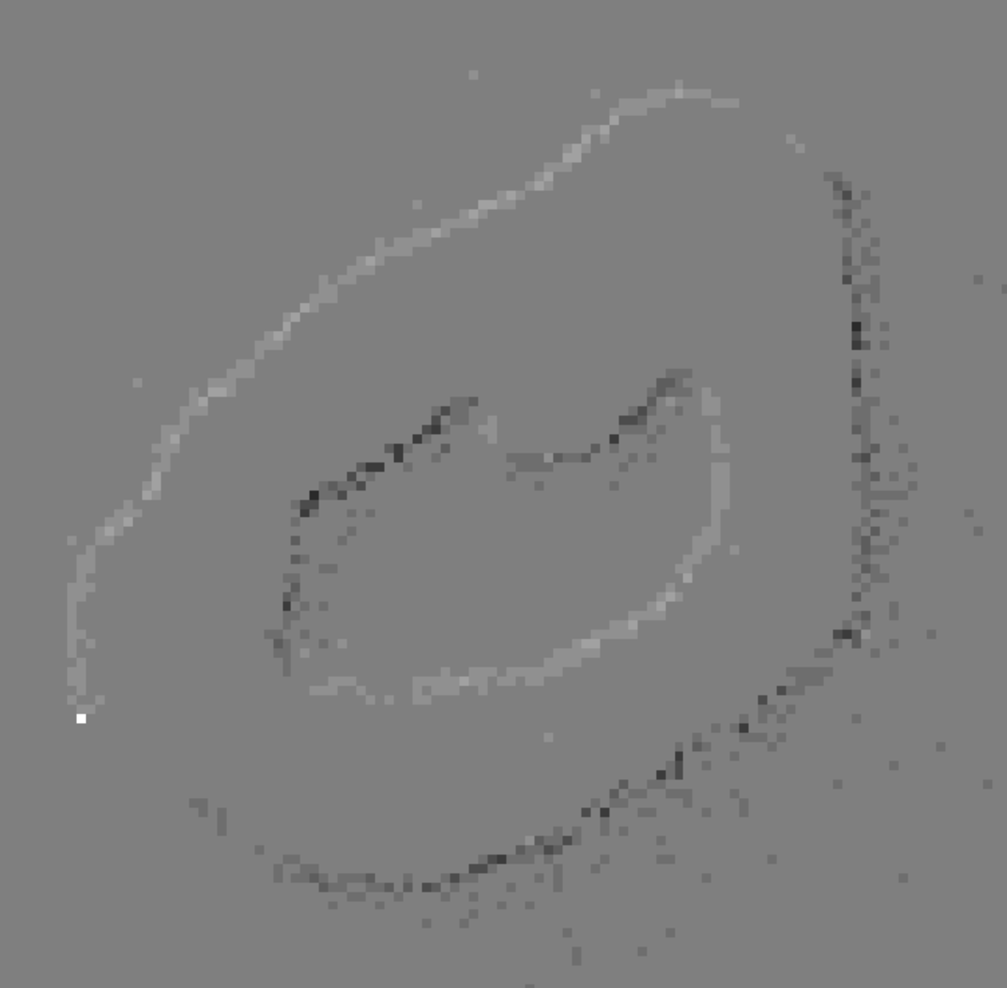
\includegraphics[width=0.22\textwidth]{images/dvs-128.pdf}
		}
		\subfloat[A snapshot of jAER playing Poissonian spike trains.]{
			\label{Fig:poisson}
			
\includegraphics[width=0.22\textwidth]{images/zero-28-2.pdf}
		}\\
		\subfloat[The raster plot of the Poissonian spike trains.]{
			\label{Fig:raster}
			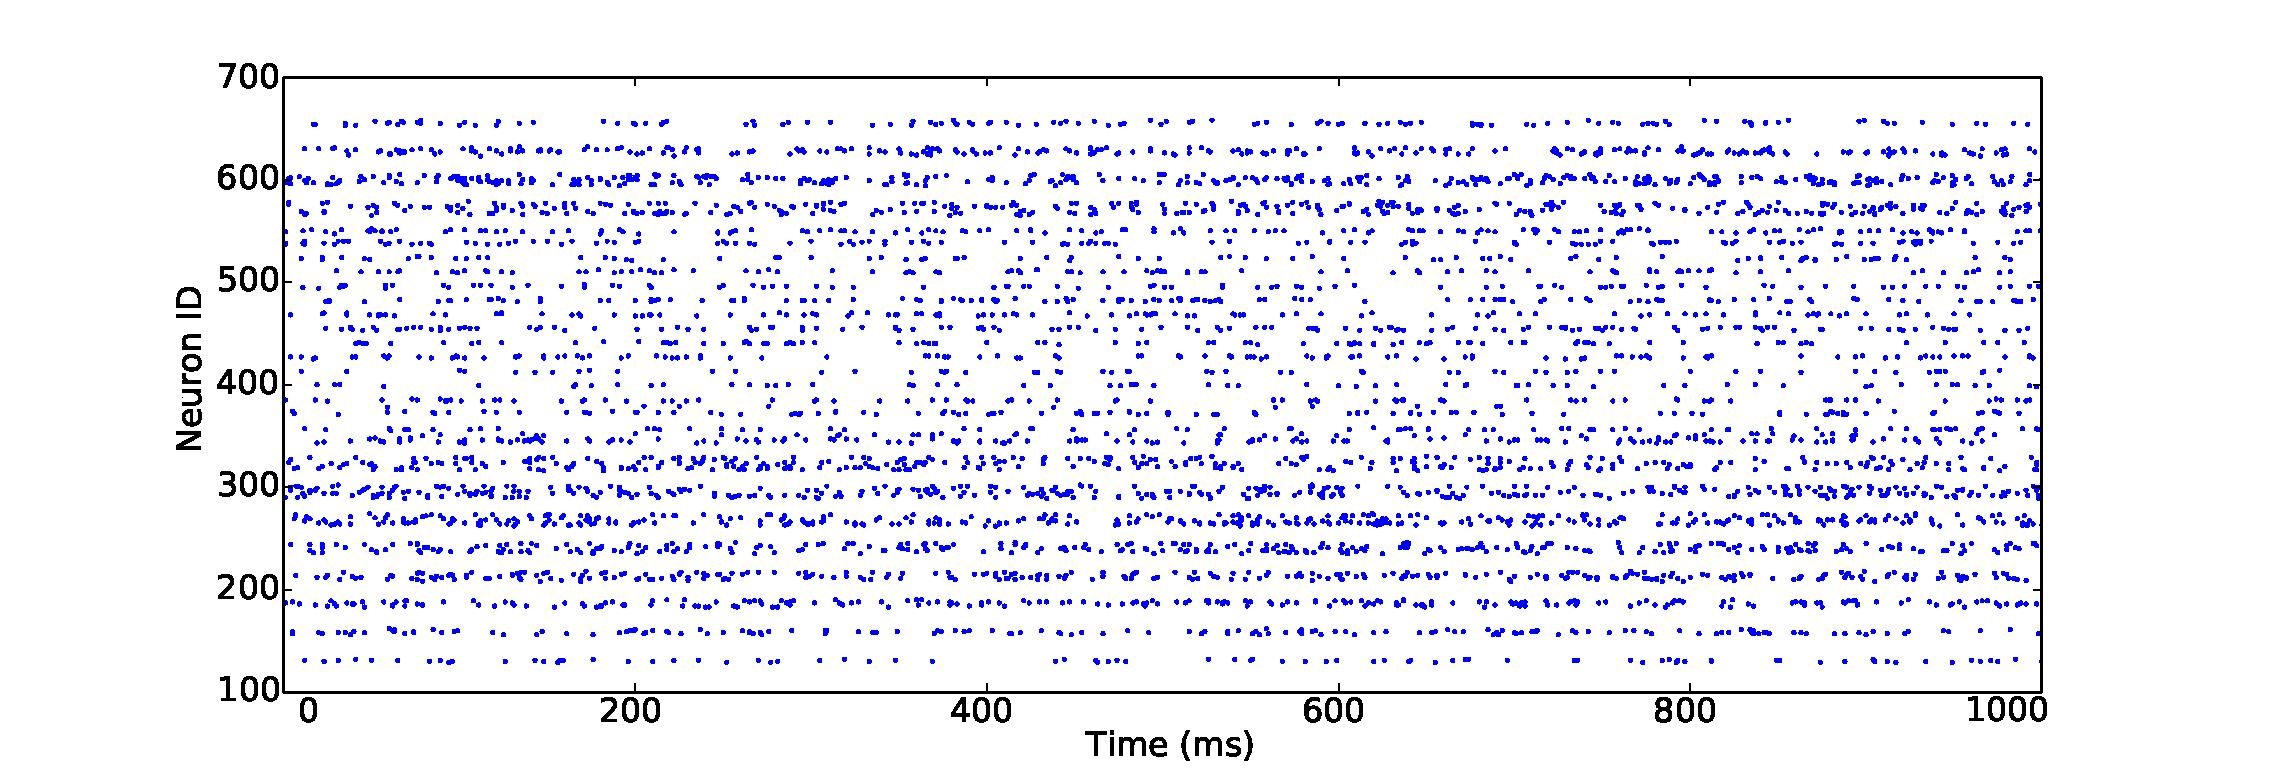
\includegraphics[width=0.48\textwidth]{images/zero.pdf}
		}
		
		\caption{
			Snapshots of jAER software playing spike presented videos.
			The same image of digit ``0'' is transformed to spikes by DVS recording and the Poissonian generation respectively.
			A raster plot of the Poissonian spike trains is also provided.}
		\label{fig:zero}
	\end{figure}
	
\section{Evaluations on Spike-Based Recognition}
	The complementary evaluation methodology is essential to assess both the model-level and hardware-level performances.
	For a network model, its topology, neuron and synapse models, and training methods are major descriptions for any kind of neural networks, including SNNs.
	While the recognition accuracy, network latency and also the biological time taken for both training and testing are specific performance measurements of a spike-based model.
	To build any SNN model on a hardware platform, its network size will be constrained by the scalability of the hardware. Neural and synaptic models are limited to the ones that are physically implemented, unless the hardware platform supports programmability.
	The accuracy of the results (e.g. CA) are naturally affected by the precision of the variable representing the membrane potential and synaptic weights.
	Any attempt to implement an on-line learning algorithm on neuromorphic hardware must be backed by synaptic plasticity support.
	Running an identical SNN model on different neuromorphic hardware platforms can not only expose if any of the previously mentioned capacities are supported, but also benchmark their performance on simulation time and energy usage.
	
	The test results of the case studies as examples using the dataset are listed in Table~\ref{tb:software_comparison} and evaluated on the proposed metrics.
	While the hardware evaluation metrics is listed in Talbe~\ref{tb:hardware_comparison}
	\begin{table}[h!]
		\caption{Hardware independent comparison}
		\begin{center}
			\bgroup
			\def\arraystretch{1.5}
			\begin{tabular}{ l c c c c }
				\begin{mycell}{0.2cm} % %\cite{Stromatias2015scalable} \\ 
				\end{mycell}  &
				\begin{mycell}{0.3cm}Pre\end{mycell} & 
				\begin{mycell}{1.5cm} Network\end{mycell} & 
				\begin{mycell}{2.5cm} Training \end{mycell} & 
				\begin{mycell}{1.5cm} Recognition \end{mycell} \\
				\hline
				
				%

				
				\begin{mycell}{0.2cm} Exp 1 \end{mycell}  & 
				\begin{mycell}{0.3cm} None \end{mycell}& % preprocessing 
				\begin{mycell}{1.5cm} FC Network, \\ LIF neurons \end{mycell}& % network
				\begin{mycell}{2.5cm} K-means clusters,\\Supervised STDP\\$18,000$~s of training \end{mycell}& % training
				\begin{mycell}{1.5cm} 92.98\%\\1~s per test\\10.70~ms latency\end{mycell}\\ % recognition
				
				
				
				\begin{mycell}{0.2cm} % %\cite{Stromatias2015scalable} \\ 
					Exp 2 \end{mycell} & 
				\begin{mycell}{0.3cm} None \end{mycell} & % preprocessing
				\begin{mycell}{1.5cm} 4-layer RBM, \\ LIF neurons \end{mycell}&  % network
				\begin{mycell}{2.5cm} Off-line trained, unsupervised \end{mycell}&  % training
				\begin{mycell}{1.5cm} 94.94\%\\16 ms latency \end{mycell} \\% recognition
				%
			\end{tabular}
			\egroup
		\end{center}
		\label{tb:software_comparison}
	\end{table}
	
	\begin{table*}[thb!]
		\caption{Hardware dependent comparison}
		\begin{center}
			\bgroup
			\def\arraystretch{1.4}
			\begin{tabular}{l c c c c c c}
				$ $ & 
				\begin{mycell}{2.0cm} System \end{mycell} & 
				%       \begin{minipage}{1.3cm}\centering Simulation type \end{minipage} & 
				
				\begin{mycell}{2.0cm} Neuron Model \end{mycell} & 
				\begin{mycell}{2.0cm}Synaptic\\Plasticity\end{mycell} &
				%       \begin{minipage}{1cm}\centering Axonal delays \end{minipage} & 
				%       \begin{minipage}{1cm}\centering Synaptic model \end{minipage} & 
				\begin{mycell}{2.0cm} Precision \end{mycell} &  
				%       \begin{minipage}{1.2cm}\centering Synaptic precision \end{minipage} & 
				%       \begin{minipage}{1.2cm}\centering Energy per SE \end{minipage} & 
				%       \begin{minipage}{1.4cm}\centering Synaptic ops per Watt \end{minipage} & 
				\begin{mycell}{2.0cm} Simulation\\Time \end{mycell} & 
				\begin{mycell}{2.0cm} Energy/Power \\Usage \end{mycell} 
				%       \begin{minipage}{1.7cm}\centering Programming front-end \end{minipage}  
				\\
				\hline
				% contents!
				
				\begin{mycell}{1.8cm} SpiNNaker \cite{stromatias2013power} \end{mycell} &
				\begin{mycell}{2.0cm} Digital, \\Scalable \end{mycell} & 
				\begin{mycell}{2.1cm}Programmable\\Neuron/Synapse,\\Axonal delay \end{mycell}& 
				\begin{mycell}{2.1cm}Programmable\\learning rule\end{mycell}& 
				\begin{mycell}{2.0cm}11- to 14-bit synapses\end{mycell} & 
				\begin{mycell}{2.0cm} Real-time \\ Flexible time resolution \end{mycell}  &
				\begin{mycell}{2.5cm} 8~nJ/SE \\54.27 MSops/W \end{mycell} \\
				%
				\begin{mycell}{1.8cm} TrueNorth \cite{merolla2014million}\end{mycell} & \begin{mycell}{2.0cm}Digital, \\Scalable \end{mycell}& 
				\begin{mycell}{2.0cm}Fixed models,\\Config params,\\Axonal delay\end{mycell}& 
				\begin{mycell}{2.0cm}No plasticity\end{mycell}& 
				\begin{mycell}{2.2cm}122 bits \\params \& states,
					%       	 per neuron
					\\ 4-bit synapse 
					\\(4 signed int + on/off state)
				\end{mycell}& 
				\begin{mycell}{2.0cm}Real-time\end{mycell}& 
				\begin{mycell}{2.0cm}46 GSops/W\end{mycell} \\
				
				%
				\begin{mycell}{1.8cm} Neurogrid \cite{benjamin2014neurogrid}\end{mycell} &
				\begin{mycell}{2.0cm}Mixed-mode,\\Scalable\end{mycell} & 
				\begin{mycell}{2.0cm}Fixed models,\\Config params\end{mycell} & 
				\begin{mycell}{2.0cm}Fixed rule\end{mycell} & 
				\begin{mycell}{2.0cm}13-bit shared \\ synapses\end{mycell} &
				\begin{mycell}{2.0cm}Real-time\end{mycell} &
				\begin{mycell}{2.0cm}941 pJ/SE\end{mycell} \\
				%
				\begin{mycell}{1.8cm} HI-CANN \cite{schemmel2010wafer}  \end{mycell} & \begin{mycell}{2.0cm}Mixed-mode,\\Scalable\end{mycell} &
				\begin{mycell}{2.0cm}Fixed models,\\Config params\end{mycell}& 
				\begin{mycell}{2.0cm}Fixed rule\end{mycell}& 
				\begin{mycell}{2.0cm}4-bit synapses\end{mycell}& 
				\begin{mycell}{2.0cm}Faster than\\ real-time\end{mycell}&
				\begin{mycell}{2.0cm}198 pJ/SE \\ 13.5 MSops/W \\(network only) \end{mycell}\\
				%
				\begin{mycell}{1.8cm} iAER-IFAT \cite{yu201265k}\end{mycell} & 
				\begin{mycell}{2.0cm}Mixed-mode,\\Scalable\end{mycell} &
				\begin{mycell}{2.0cm}Fixed models,\\Config params\end{mycell}& 
				\begin{mycell}{2.0cm}No plasticity\end{mycell} &  
				\begin{mycell}{2.0cm}Analogue neuron/synapse\end{mycell} & 
				Real-time& 
				20GSops/W
				%dummy update text
			\end{tabular}
			\egroup
		\end{center}
		\label{tb:hardware_comparison}
	\end{table*}

\section{Case Studies}
We present two recognition SNN models working on the Poissonian subset of the NE15-MNIST dataset.
Their network components, training and testing methods are described in the paper~\cite{Liu2015Bench} (under corrections of the reviews) according to the evaluation methodology stated above.
The specific spike-based evaluations on input event rates and/or responding latency are also provided. 
Meanwhile, as tentative benchmarks the models are implemented on SpiNNaker to assess the performance against software simulators.
Presenting proper benchmarks for vision recognition systems is still under investigation, the case studies only make first attempt.
	\subsection{2-Layer STDP}
	The case study is a simple two-layered network where the input neurons receive Poissonian presented spike trains from the dataset and form an FC network with the decision neurons.
	The model utilises LIF neurons, and the parameters are all with biological means.
	
	In order to fully assess the performance, different settings have been configured on the network, such as network size, input rate and testing images duration.
	There are two layers in the model: 28$\times$28 input neurons fully connect to 100 decision neurons.
	Each decision neuron responds to a certain template of a digit.
	In the standard configuration, there are 10 decision neurons answering to the same digit with slightly different templates, e.g. altogether 10$\times$10 decision neurons.
	Those templates are embedded in the connection weights between the two layers.
	Fig.~\ref{Fig:train} shows how the connections to a single decision neuron are tuned.
	
	The training set of $60,000$ hand written digits are firstly classified into 100 classes, 10 subclasses per digit, using K-means clusters.
	So the images in a certain subclass are used to train one corresponding decision neuron.
	The firing rates of the input neurons are assigned linearly according to their intensities and normalised with a total firing rate of $2,000$~Hz.
	All the images together are presented for $18,000$~s (about 300~ms per image) during training and at the same time a teaching signal of 50~Hz is conveyed to the decision neuron to trigger STDP learning.
	The trained weights are plotted in accordance with the positions of the decision neurons in Fig.~\ref{Fig:test}.
	\begin{figure}[thb!]
		\centering
		\subfloat[Training model of a single decision neuron.]{
			\label{Fig:train}
			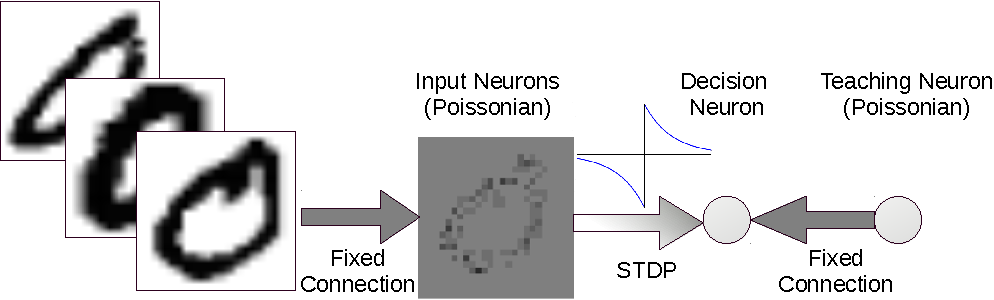
\includegraphics[width=0.48\textwidth]{images/training.pdf}
		} \\
		
		\centering
		
		\subfloat[Testing model of the spiking neural network.]{
			\label{Fig:test}
			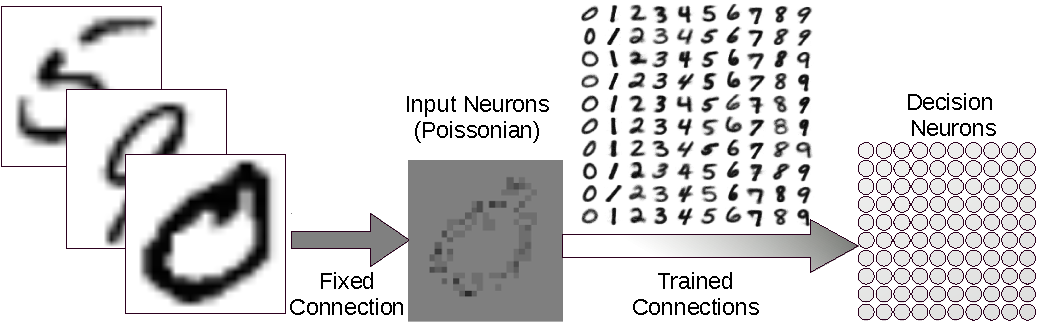
\includegraphics[width=0.48\textwidth]{images/testing.pdf}
		}
		
		\caption{The training and testing model of the two-layered spiking neural network.}
		\label{fig:model}
	\end{figure}
%	\subsubsection{Testing}

	After training the weights of the plastic synapses are set to static, keeping the state of the weights at the last moment of training.
	The feed-forward testing network is shown in Fig.~\ref{Fig:test} where Poissonion spike trains are generated the same way as in the training with a total firing rate of $2,000$~Hz per image.
	The input neurons convey the same spike trains to every decision neuron through its responding trained synaptic weights. 
	Every testing image ($10,000$ images in total) is presented once and lasts 1~s with a silence of 200~ms between them.
	The output neuron with the highest firing rate decides what digit was recognized.
	
	Among different network configurations, the network of 500 decision neurons (50 clusters per digit) reaches the highest recognition rate.
	%The recognition accuracy reaches the highest (92.98\%) when 50 patterns are trained per digit.
	The network achieved a CA of 92.98\% and average latency of 10.70~ms, and the simulation costs SpiNNaker 0.41~W on power use and $4,920$~J on energy use~\ref{fig:energy}.
	
	\begin{table}[h]
	\caption{Comparisons of NEST (N) on a PC and SpiNNaker (S) performances.}
	\begin{center}
	\begin{tabular} {r|c|c|c|c|c|c}
		 Clusters
		 &\multicolumn{2}{c|}{Accuracy (\%)}  &\multicolumn{2}{c|}{Simulation (s)}
		 &\multicolumn{2}{c}{Power Use (W)}   \\
		 \cline{2-7}
		 per digit
		& N & S & N & S & N & S\\
	    \hline
	    1 & 79.62 & 79.50 & 554.77 & \multirow{5}{*}{$12,000$} & \multirow{5}{*}{ 21.0 } & 0.38 \\
	    10 & 91.29 & 91.43 & 621.74 &   &   & 0.38 \\
	    50 & 92.98 & 92.92 & $1,125.12$ &   &   & 0.41 \\
	    100 & 87.27 & 86.83 & $1,406.01$ &   &   & 0.44 \\
	    1000 & 89.65 & 89.74 & $30,316.88$ &   &   & 1.50 \\
	
	\end{tabular}
	\label{tbl:compare}
	\end{center}
	\end{table}
	
	\begin{figure}[hbt!]
		\centering
		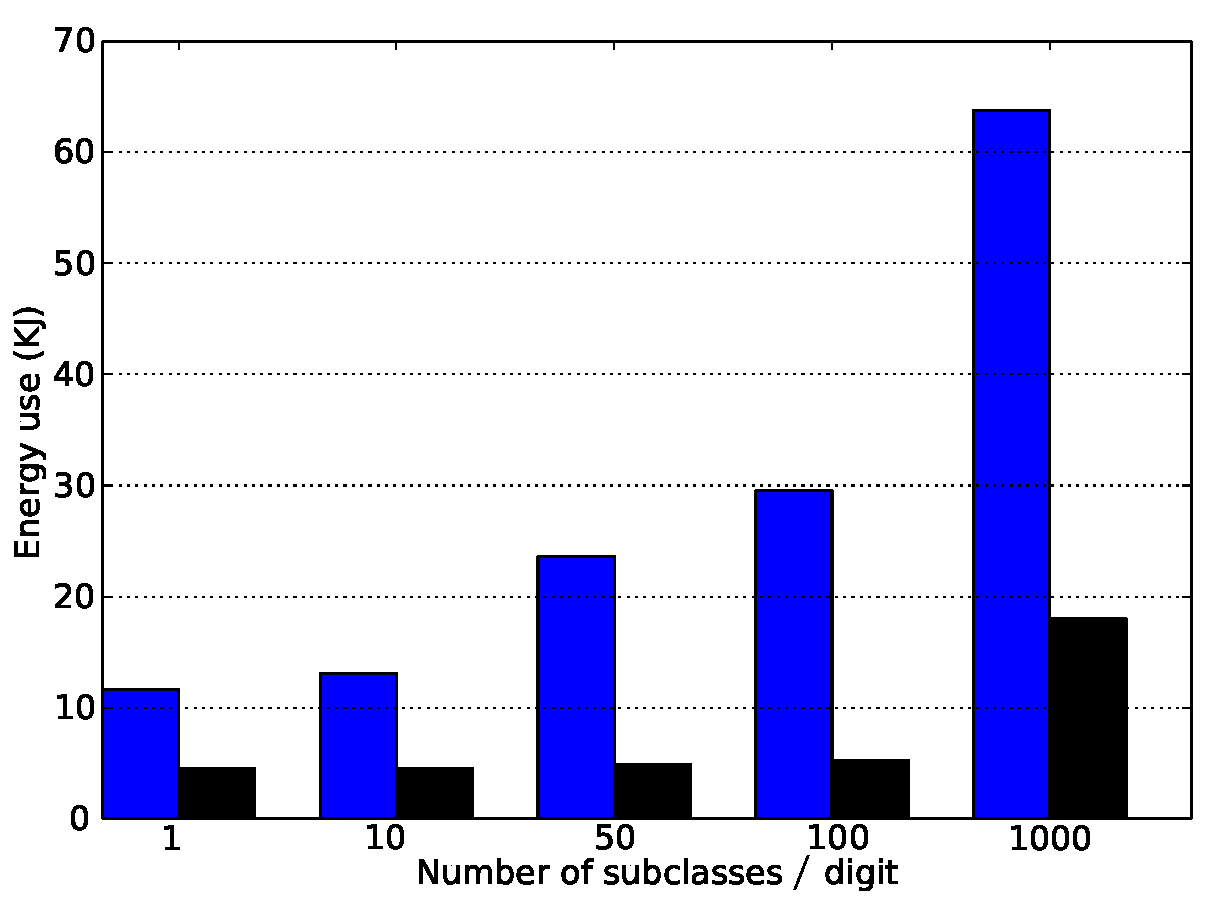
\includegraphics[width=0.4\textwidth]{images/energy.pdf}
		\caption{Energy usages of different network size both using NEST (blue) on a PC and SpiNNaker (black).}
		\label{fig:energy}
	\end{figure}
	
	\subsection{Case Study II}
	Paper~\cite{o2013real} proposed a method to map off-line trained DBNs into a spiking neural networks and take advantage of the real-time performance and energy efficiency of neuromorphic platforms. 
	For this work we used an off-line trained spiking DBN with a 784-500-500-10 network topology.
	Simulations take place on a software spiking neural network simulator named Brian~\cite{goodman2008brian} and results are verified on the SpiNNaker platform.
	
	A similar experiment to the one presented for the Case Study I was performed; its purpose was to establish the relation that input spike rates hold with latency and classification accuracy.
	The input rates were varied from 500~Hz to $2,000$~Hz and the results are summarised in Figure~\ref{Fig:brianLatency}. Simulations ran in Brian for all $10,000$ MNIST digits of the testing set and for 4 trials. 
	The mean classification latency for the particular spiking DBN on SpiNNaker is 16~ms which is identical to the Brian simulation seen in Figure~\ref{Fig:brianLatency}.
	
	\begin{figure}[hbt!]
		\centering
		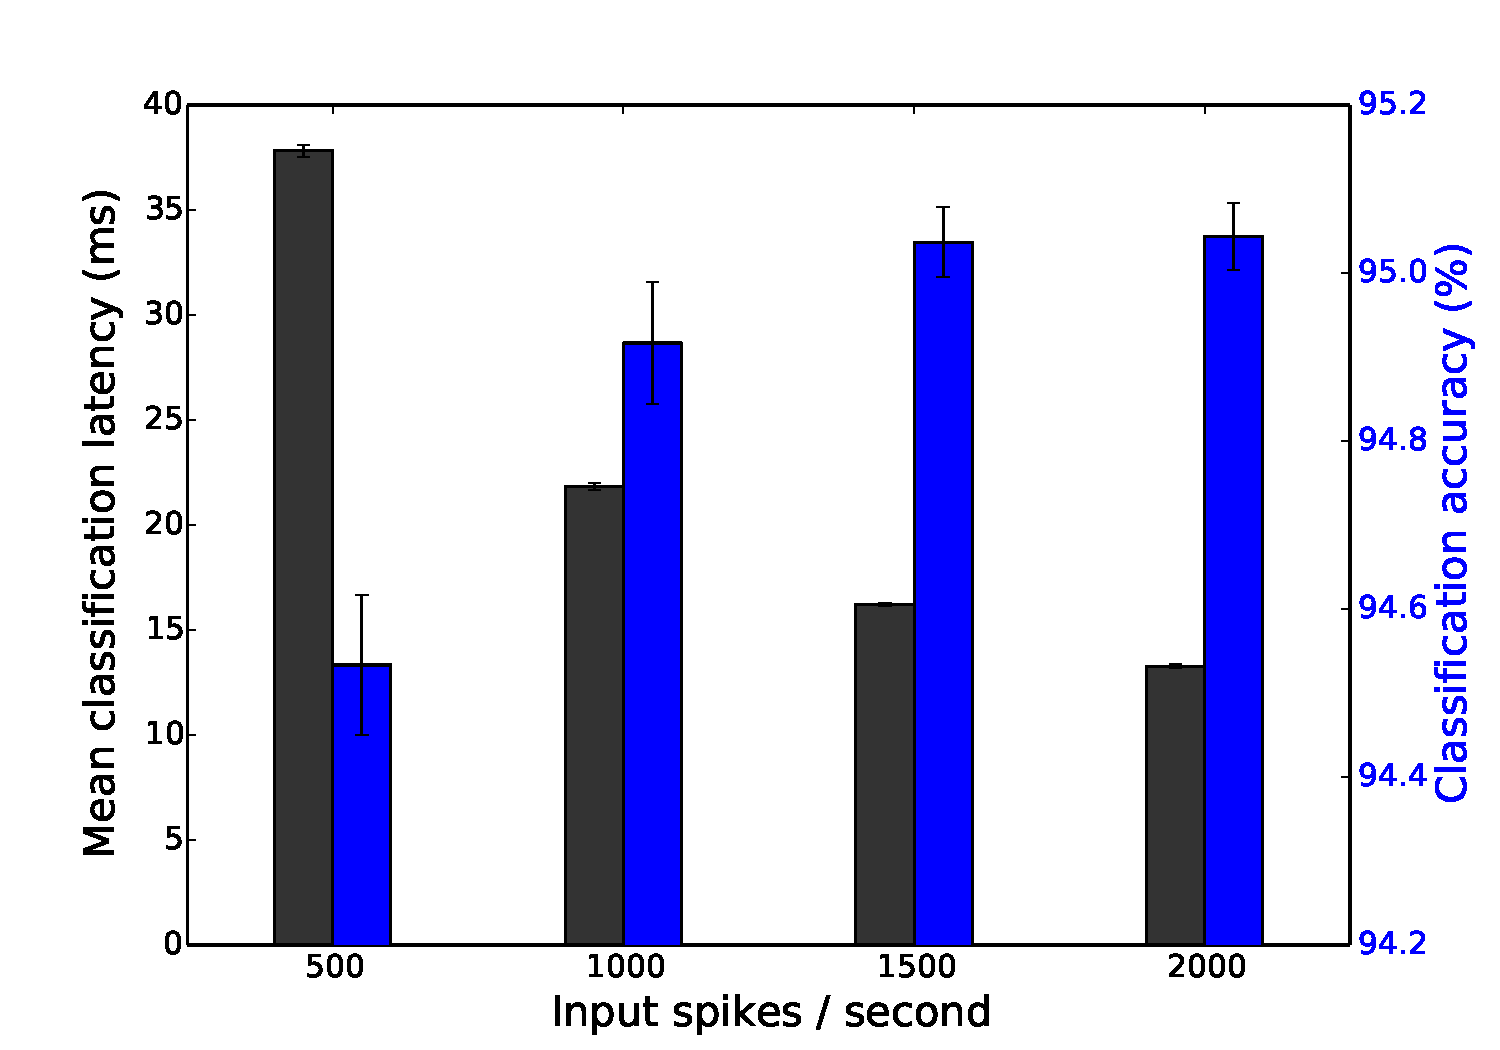
\includegraphics[width=0.4\textwidth]{images/evan/latencyCAfiringrate.pdf}
		\caption{Mean classification latency (black) and classification accuracy (blue) as a function of the input spikes per second for the spiking DBN. Results are averaged over 4 trials, error bars show standard deviations.}
		\label{Fig:brianLatency}
	\end{figure} 
	
\section{Preliminary and Future Work}
	One of the main research in the future is to apply biologically-inspired learning algorithms to the SDBN thus to provide the comparison with the state-of-the-art of the deep learned image recognition.
	The event-based learning will benefit from exploiting neuromorphic hardware platforms to train a large-scale DBN model in real time.
	The comparison on time and energy cost of DBN learning between conventional ANN and event-based SNN will be of interest in the neuromorphic community. 
	The current work starts from layer-by-layer pre-training of RBMs and the fine-training of a DBN, and future work will focus on applying spiking learning rules to DBN training, see Gantt chart Figure~\ref{fig:gannt}.
	This work is accumulatively written in my personal report~\cite{liu2015sdbn}. 
	
	Works done: (* indicates potential research)
	\begin{enumerate}
		\item Contrastive Divergence (CD)
			\begin{enumerate}
				\item Product of Experts Problem (PoE)
				\item Markov Chain Monte Carlo Sampling
				\item Gibbs Sampling
				\item CD Instead of Kullback-Leibler (KL) *
			\end{enumerate}	
		\item RBM
			\begin{enumerate}
				\item Objective Function
				\item CD with 1-Step Gibbs Sampling
				\item CD Validation Methods *
				\item Comparison of $CD_1$ and $CD_k$ *
			\end{enumerate}
		\item DBN
			\begin{enumerate}
				\item The Probabilistic Model *
				\item Greedy Algorithm
				\item Fine Training
				\item Practical Training Configurations *
			\end{enumerate}	
	\end{enumerate}			
	
	The future work will firstly reproduce the recursive network Neftci and etc. proposed~\cite{neftci2013event} for training SRBM using event-driven contrastive divergence (eCD).
	It will followed by improving and formalisation of their methods and proposing new algorithms.
	The fine-training on pre-trained layered SRBMs in an SDBN will be studied afterwords, and SpiNNaker on-line trained models will be provided as benchmarks.

		\begin{figure*}[hbt]
			\centering
			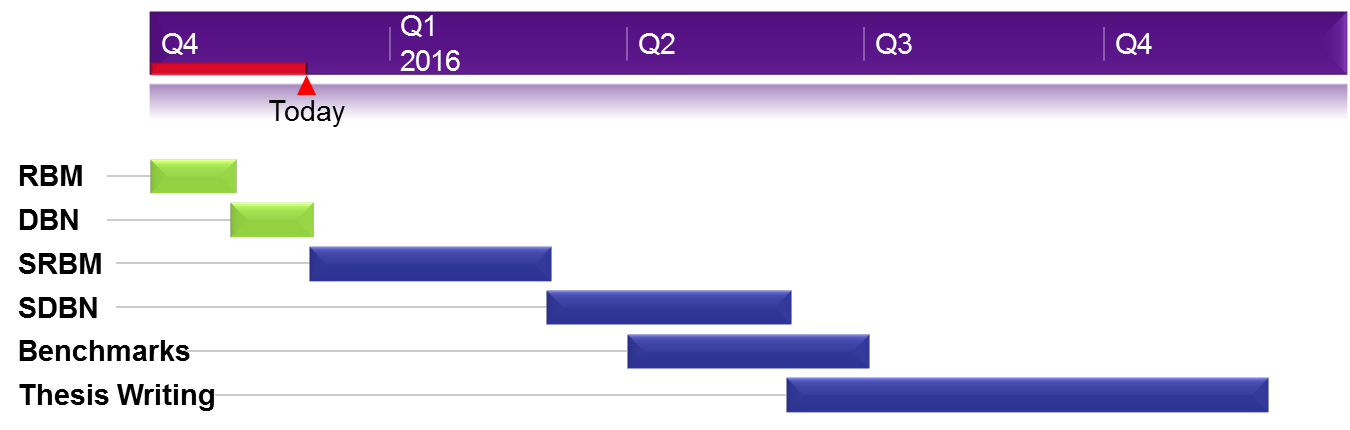
\includegraphics[width=0.7\textwidth]{images/gantt.png}
			\caption{Gantt Chart of the future work.}
			\label{fig:gannt}
		\end{figure*}



\bibliography{ref}    % this causes the references to be listed
\bibliographystyle{ieeetr}

\begin{appendices}
	\section{Thesis Outline}
	\label{app:thesis}
	The following section-level outline gives the planned thesis structure for this project.
	Sections which are reliant on upcoming work are indicated with a star (*);
	\begin{enumerate}
		\item Introduction
		\item Background
			\begin{enumerate}
				\item Neural Network on Image Recognition
				\item Neuron Models and Spiking Neural Network
				\item Spiking Neural Network Simulation
				\item Neuromorphic Simulators
			\end{enumerate}	
		\item Related Works
			\begin{enumerate}
				\item Vision Databases and Benchmarks
				\item Deep Neural Networks
				\item Spike-Based Image Recognition
				\item Real-Time Neuromorphic Vision System
			\end{enumerate}
		\item Benchmarking Spike-Based Visual Recognition
			\begin{enumerate}
				\item Database
				\item Evaluation Methodology
			\end{enumerate}
		\item Spiking Deep Belief Network
			\begin{enumerate}
				\item Restricted Boltzmann Machine  
				\item Deep Belief Network
				\item Spiking RBM and DBN *
				\item Formalisation of SDBN *
%					\begin{enumerate}
%					\item Mean Field Theory
%					\item Synaptic Learning
%					\end{enumerate}	
			\end{enumerate}	
		\item Benchmarks
			\begin{enumerate}
				\item STDP Learned 2-Layer Network
				\item Spiking DBN *
				\item Off-line Trained Convolutional Network *
			\end{enumerate}	
		\item Discussions *
			\begin{enumerate}
				\item Benefits of Spike-based Processing *
				\item Scalability of Hardware SDBN *
				\item Future NE Database Development *
			\end{enumerate}					
		\item Future Work *
			\begin{enumerate}
				\item SDBN Toolbox on SpiNNaker *
%				\item Learning on Spiking Convolutional Network  *
				\item Video-Based Recognition and Benchmarks *
				\item Natural Language Processing and Benchmarks *
%				\item Benchmarking Real-Time Neuromorphic Systems
			\end{enumerate}					
	\end{enumerate}	
\end{appendices}

\end{document}